\documentclass[Space_Shuttle_Ultra_Manual.tex]{subfiles} 
\begin{document}

\section{UPPER STAGES}
\begin{multicols*}{2}
\label{sec:upper-stages}
\renewcommand{\cfttoctitlefont}{\bf}
\localtableofcontents
\noindent
\\
Currently SSU supports the 2 biggest and more powerful Space Shuttle upper stages$\colon$ the Centaur and the Inertial Upper Stage. These 2 upper stages allow the Space Shuttle Ultra add-on to launch payloads to anywhere from GEO to the depths of the Solar System.
\end{multicols*}

\subsection{Centaur}
\begin{multicols*}{2}
\renewcommand{\cfttoctitlefont}{\bf}
\localtableofcontents
\subsubsection{Description}
\noindent
In the 1980s, NASA modified the Centaur upper stage with the intent to use it aboard the Space Shuttle.
\\
TODO <insert side-by-side images of both centaurs attached to the CISS in raised position>
\\
Two versions were developed$\colon$ the Centaur G version was primarily for GEO satellite deployment missions, and the larger, more powerful Centaur G Prime for interplanetary payloads. In the aftermath of the Challenger accident, the Centaur was no longer considered safe enough to be used by the Space Shuttle, and so it was abandoned.
\\
Thrust is provided by 2 RL-10 engines, and the Attitude Control System (ACS) allows 3-axis control of the stage, and also translation in the +Z direction (forward).

\subsubsection{Performance (Centaur G)}
TODO performance
\begin{figure}[H]
  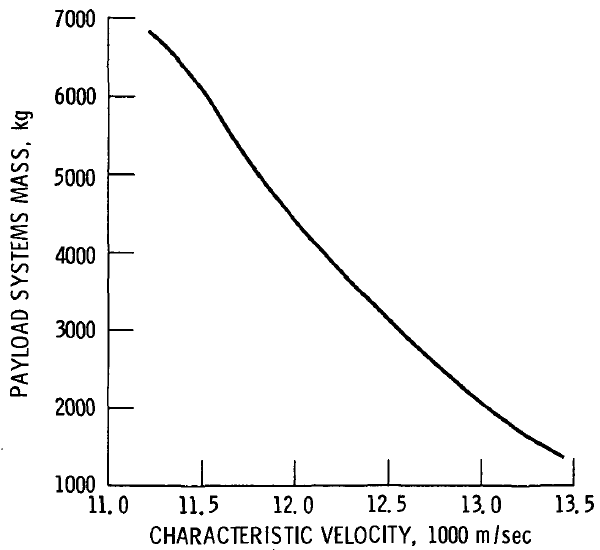
\includegraphics[width=0.5\textwidth]{Gpayload.png}
  \caption{Centaur G Payload capability}
  \label{fig:Gpayload}
\end{figure}

TODO payload envelope

\subsubsection{Performance (Centaur G Prime)}
TODO performance
\begin{figure}[H]
  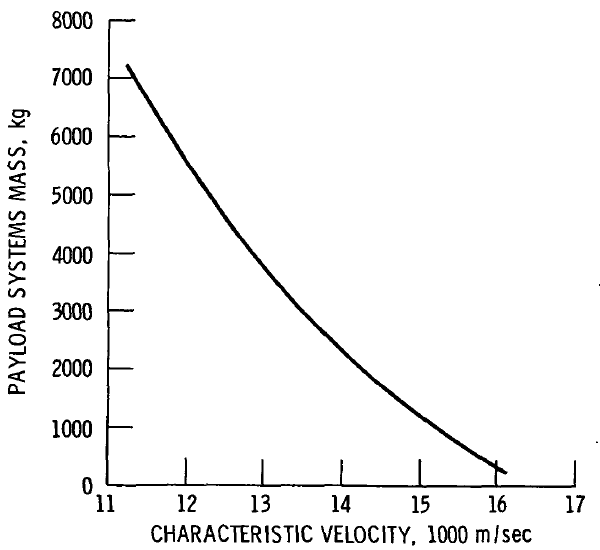
\includegraphics[width=0.5\textwidth]{GPpayload.png}
  \caption{Centaur G Prime Payload capability}
  \label{fig:GPpayload}
\end{figure}

TODO payload envelope

\subsubsection{Centaur Integrated Support Structure}
The Centaur Integrated Support Structure (CISS) is the interface between the Centaur stage and the orbiter vehicle. The CISS has a tilt table, to which the Centaur is attached, allowing it to be raised above the payload bay for deployment.
\\
TODO <insert image of empty CISS in PLB>

\subsubsection{Deployment sequence}
The deployment sequence is similar for both Centaur versions, and is controlled by panel L12.
\\
TODO
\\
Inhibits are placed on the operation of the ACS and of the RL-10 engines, as to protect the orbiter vehicle. At deployment, timers are started to remove those inhibits. The status of those timers is displayed in the HUD, as well as the remaining ACS propellant.

\subsubsection{Autonomous flight control}
After separation from the CISS and the engine inhibits have been removed, the Centaur is controlled by using the standard Orbiter keys. Currently there are no restrictions on the number of times the RL-10 engines can be started.
\\
After all the necessary burns are performed, payload separation is done by pressing the ''Ctrl+J'' key combination.

\end{multicols*}

\newpage

\subsection{Inertial Upper Stage}
\begin{multicols*}{2}
\renewcommand{\cfttoctitlefont}{\bf}
\localtableofcontents
\subsubsection{Description}
\noindent
The Inertial Upper Stage, or IUS, is a 2-stage solid propellant vehicle used in several Space Shuttle missions to boost satellites into GEO and space probes into Earth escape trajectories.
\\
TODO <insert image of IUS attached to the ASE in raised position>
\\
Thrust is provided by one Solid Rocket Motor (SRM) in each stage, and the Reaction Control System (RCS) allows 3-axis control of the stage, and also translation in the +Z direction (forward).
\\
The IUS can be installed in the payload bay in 2 possible positions: the forward position or the aft position (for large payloads). The position choice is defined in the mission file (section \ref{sec:mission-files}).

\subsubsection{Performance}
TODO performance
\\
TODO payload envelope

\subsubsection{Airborne Support Equipment}
The Airborne Support Equipment (ASE) is the interface between the IUS and the orbiter vehicle. The ASE has a tilt table, to which the IUS is attached, allowing it to be raised above the payload bay for deployment.
\\
TODO <insert image of empty ASE in PLB>

\subsubsection{Deployment sequence}
The IUS deployment sequence is controlled by panel L10.
\\
TODO
\\
Inhibits are placed on the operation of the RCS and of the $1^{st}$ stage motor, as to protect the orbiter vehicle. At deployment, timers are started to remove those inhibits. The status of those timers is displayed in the HUD, as well as the remaining RCS propellant.

\subsubsection{Autonomous flight control}
After separation from the ASE and the engine inhibits have been removed, the IUS is controlled by using the standard Orbiter keys. Once ignited, the solid rocket motors will burn to depletion. After $1^{st}$ stage burnout, its separation is done by pressing the ''Ctrl+G'' key combination. After $1^{st}$ stage separation, the Extendable Exit Cone in the $2^{nd}$ stage will automatically deploy.
\\
Due to the nature of the solid propellant motors, fine control of the delta-V is impossible during the burn, so the propellant quantity must be carefully set using the offload capability provided by the appropriate scenario file parameters. The ''LOAD\_STAGE1'' and ''LOAD\_STAGE2'' parameters, followed by a number between 0.5 (50\% offload) and 1.0 (0\% offload), allow to control the initial propellant mass of each SRM. In addition the RCS can be used for velocity fine tuning after the SRM burns.
\\
After all the burns are performed, payload separation is done by pressing the ''Ctrl+J'' key combination.
\end{multicols*}
\end{document}